\documentclass[10pt,twocolumn,letterpaper]{article}

\usepackage{cvpr}
\usepackage{times}
\usepackage{epsfig}
\usepackage{graphicx}
\usepackage{amsmath}
\usepackage{amssymb}
\usepackage{tabularx}
\usepackage{multirow}

% Include other packages here, before hyperref.

% If you comment hyperref and then uncomment it, you should delete
% egpaper.aux before re-running latex.  (Or just hit 'q' on the first latex
% run, let it finish, and you should be clear).
\usepackage[breaklinks=true,bookmarks=false]{hyperref}

\cvprfinalcopy % *** Uncomment this line for the final submission

\def\cvprPaperID{****} % *** Enter the CVPR Paper ID here
\def\httilde{\mbox{\tt\raisebox{-.5ex}{\symbol{126}}}}

% Pages are numbered in submission mode, and unnumbered in camera-ready
%\ifcvprfinal\pagestyle{empty}\fi
\setcounter{page}{1}
\begin{document}

%%%%%%%%% TITLE
\title{CNNs for Single Image Super Resolution}

\author{Michele Bortone\\
{\tt\small michele.bortone@studenti.unipd.it}
% For a paper whose authors are all at the same institution,
% omit the following lines up until the closing ``}''.
% Additional authors and addresses can be added with ``\and'',
% just like the second author.
% To save space, use either the email address or home page, not both
\and
Alessio Lazzaron\\
{\tt\small alessio.lazzaron@studenti.unipd.it}
}

\maketitle
%\thispagestyle{empty}

%%%%%%%%% ABSTRACT
\begin{abstract}
   	Super-resolution is the process to create high-resolution images from low-resolution images.
   	Single image super-resolution (SISR), refers to the goal of recovering one high-resolution image from one low-resolution image.\\
    In this study we report a comparison between some convolutional neural networks architectures that can solve this task, analyzing its performance. Our goal was to determine if the increase in complexity between the various architectures,  would lead to an increase in performance.\\
    We have analyzed three different architectures and evaluated performance with common image compression quality metrics.
    
\end{abstract}

%%%%%%%%% BODY TEXT
\section{Introduction}

	In most computer vision tasks, high resolution images are usually desired for image processing and analysis. Single Image Super Resolution is widely used in some medical imaging applications (e.g. magnetic resonance imaging), and security and surveillance imaging as well. Moreover, object detection problems can be accomplished using Super-resolution  which helps when low resolution is caused by the long distance between the target and the imaging sensor and objects are too small.
	Super-resolution (SR) refers to the task of restoring high-resolution images (HR) from one or more low-resolution (LR) observations of the same scene. According to the number of input LR images, the SR can be classified into single image super-resolution (SISR) and multi-image super-resolution (MISR). Compared with MISR, SISR is much more popular because of its high efficiency.
	Many SISR methods have been studied in the digital age, including interpolation tecniques such as Nearest neighbor or bicubic.\\
	Recent popular methods are based on neural networks and most architectures studied for this task are Convolutional Neural networks and Deep Generative models.\\
	The deep learning models capability is particularly suitable for this type of task because simpler approaches like bicubic interpolation use only local information in an LR image to compute pixel values in the corresponding SR image, deep learning approaches, on the other hand, learn mapping functions from LR images to HR images from a large number of examples.\\
	
\section{Related work}
	Deep learning can be used to estimate the high-resolution image given a low-resolution image. By using the HR image as a target (or ground-truth) and the LR image as an input, we can treat this like a supervised learning problem. There are a lot of approaches to affront this problem however most of them use CNNs because they get better performances.  Some approaches are listed below and represent a broad outline of the current state of the art.
\subsection{Pre-upsampling}
	In this method, the low-resolution images are first interpolated to obtain a “coarse” high resolution image. Now, CNNs are used to learn an end-to-end mapping from the interpolated low resolution images to the high resolution images. The intuition was that it may be easier to first upsample the low-resolution images using traditional methods (such as Bicubic interpolation) and then refine the resultant than learn a direct mapping from a low-dimensional space to a high-dimensional space. The advantage is that since the upsampling is done by traditional methods, the CNN only needs to learn how to refine the coarse image, which is simpler.\\
	In our comparison, we implemented and analyzed two pre-upsampling networks, that are SRCNN \cite{dong2014image} (Super Resolution Convolutional Neural Network) and VDSR \cite{kim2015accurate} (Very Deep Super Resolution).
\subsection{Post-upsampling}
	This method works in reverse way respect to the previous one, indeed the low-resolution images are passed to the CNNs as such. Upsampling is performed in the last layer using a learnable layer. The advantage of this method is that feature extraction is performed in the lower dimensional space (before upsampling) and so the computational complexity is reduced. Also, by using an learnable upsampling layer, the model can be trained end-to-end.\\
	This network architecrture is suitable when we are interested to produce the output quickly because we can skip the pre-upsampling process.
	In this this report we have compared FSRCNN \cite{dong2016accelerating} (Fast Super Resolution Convolutional Neural Network) with the two Pre-upsampling CNNs cited above.
\subsection{Progressive upsampling}
The above approaches use only a single upsampling convolution to not increase the computational complexity. This makes the learning process harder for large scaling factors. To avoid it these models  use a cascade of CNNs to progressively reconstruct high resolution images. By decomposing a difficult task into simpler tasks, the learning difficulty is greatly reduced and better performance can be obtained.
\subsection{Iterative Up and Down sampling}
Another popular model architecture is the hourglass structure that alternating between the process of upsampling and downsampling. These models can better find the deep relations between the LR-HR image pairs and thus provide higher quality reconstruction results.
\subsection{Generative Adversarial Networks (GANs)}
This type of network have been increasingly used for several image based applications including Super Resolution. GANs typically is composed of two neural networks: the Generator and the Discriminator, that dueling each other in a zero-sum game. Given a set of target samples, the Generator tries to produce samples that can fool the Discriminator into believing they are real. The Discriminator tries to recognize the real (target) samples from fake (generated) samples. At the end we obtain a Generator that is really good at generating samples similar to the target samples.

\section{Dataset}
For our purpose we use three different dataset, the first is \textit{T91} that is the smallest dataset, it contains 91 mixed images of small size that representing fruits, vegetables, objects and people, every images is in Bitmap format. The second is \textit{General100} that contains 100 bmp-format images with no compression. The size of these 100 images ranges from 710 x 704, the largest, to 131 x 112, the smallest. And the third dataset is \textit{Berkeley Segmentation Dataset (BSDS200)}, ot contain 200 images and it is created for developing new boundary detection algorithms and for developing a benchmark for that task. For each neural network that we implement, we also adjust the number of epochs for the training phase, in fact, since the size of the datasets were different it was necessary to customize this hyperparameters to have, more or less, the same performances on the validation test and avoid overfitting. The validation set is obtained by split the dataset in two parts: the biggest one, almost the 80\% of the dataset, for the training set, and the rest 20\% for the validation set. However using different type of training set didn't change the models performance so much.\\
To testing the performance of the models and to understand how much the models are able to reconstruct from the low-resolution images to high resolution images we use, as testing dataset, \textit{Set5} and \textit{Set14} that are common evaluation dataset  for Super Resolution task and contains various images of buildings to animal faces.\\
Official web pages of SRCNN, FSRCNN and VDSR provide all datasets used.
We don’t use directly the dataset but we apply some preprocessing. First off all we convert the training set’s images from RGB into YCbCr format because the models is training with only the luma, the brightness, of the images. After this, we normalize the images in order to have floating point values between 0 and 1, so in this way we make the convergence of the loss function faster. The low-resolution images is made by down and up sampling the images, inside the dataset, with a bicubic interpolation and we analyze the model’s performance with different scale factors.\\
In order to perform training operations with larger dataset we do some data augmentation. 
We crop small images called patches from each images in the training set. Patches are overlapping sub-images densely cropped from the original image with low size. The stride, which controls how many images are cropped, and size are hyperparameters.\\
Patch extraction is the process of extracting a large set of small image patches,  from a single larger image. This type of data augmentation is frequently used in image-to-image regression problems such as Super Resolution, where networks can be trained on very small input image sizes.
Patch extraction is widely used  in recent Super Resolution methods.\\
Also in deep models we use rotated images to create a larger dataset for the training phase.\\


\section{Method}
\begin{figure*}[]
	\centering
	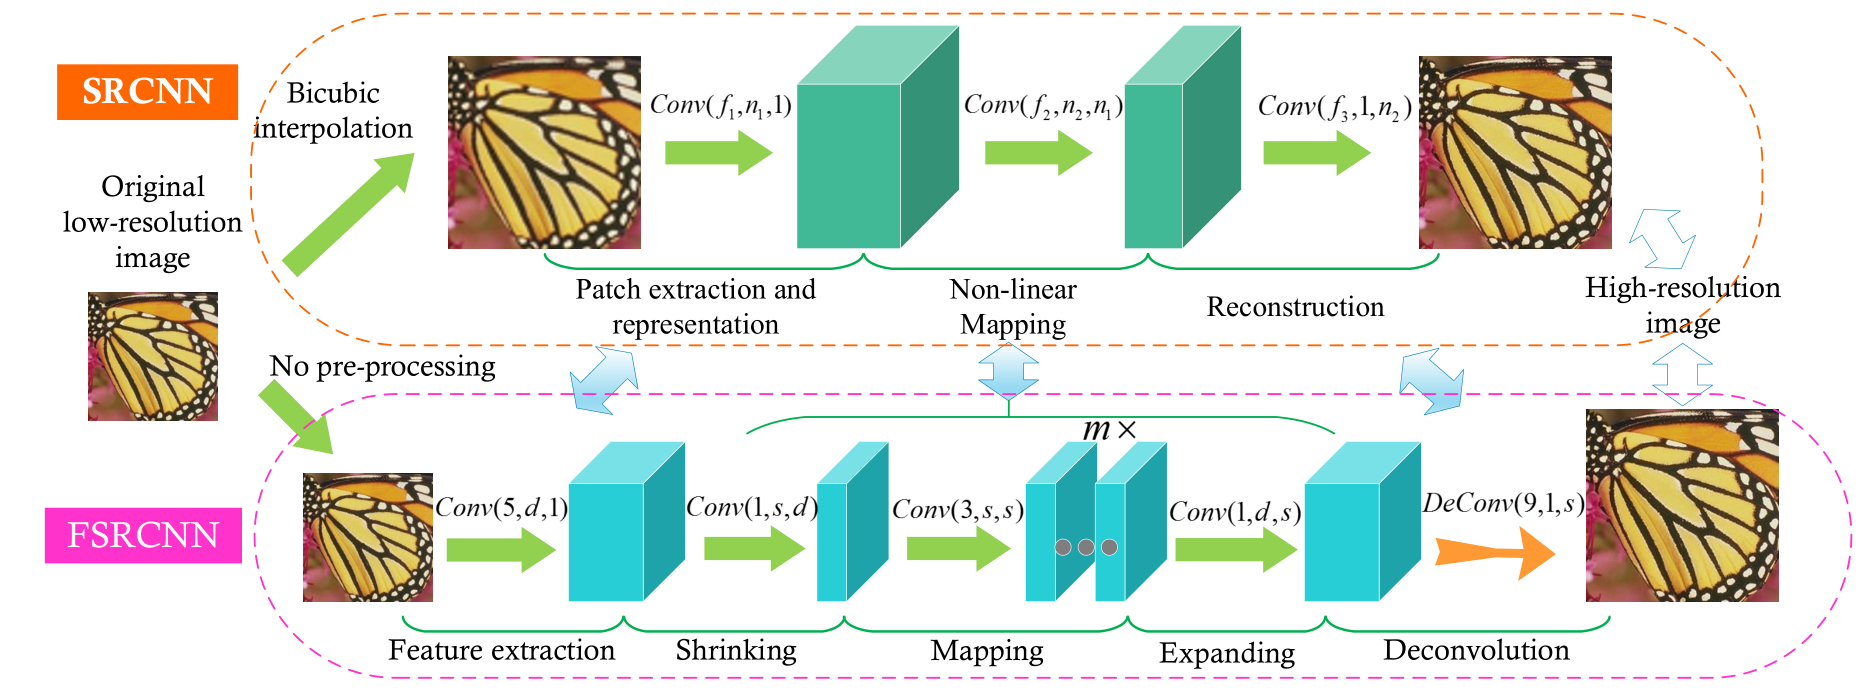
\includegraphics[width=\textwidth]{img/fsrcnn.png}
	\caption{Comparison between SRCNN and FSRCNN architectures \cite{dong2014image}}
	\label{fsrcnn}
\end{figure*}

We want to verify if the complexity of the model increases also its performance do too. So we implement three convolutional neural network that are different for the complexity of the architecture.
\subsection{SRCNN}
The Super Resolution CNN \cite{dong2014image} is relatively simple and can see as an ordinary CNN that can approximates the complex mapping between the LR and HR spaces in an end-to-end way
As shown in figure \ref{fsrcnn}, SRCNN is composed by three main parts:
\begin{itemize}
	\item \textbf{Patch extraction and representation:} extracts patches from the low-resolution image  and represents each patch as a high-dimensional vector;
	\item \textbf{Non-linear mapping:} maps each high-dimensional vector into another high-dimensional vector;
	 \item \textbf{Reconstruction:} aggregates the above high-resolution patch representations to generate the final high-resolution image;
\end{itemize}
So SRCNN has only three layer where the first layer has 64 filters and each of them as a dimension of 9x9, the second layer has 32 filters with dimension 1x1 and the output layer has only one filter with dimension 5x5. Every layer not have padding and for the first two layers we use a relu activation function and for the last layer we adopt a linear activation function. The loss that the model want to minimize is the mean square error, between the low resolution images and the output high resolution images, using stochastic gradient descent with the standard backpropagation. More precisely we adopt Adam as optimization algorithm 

\subsection{FSRCNN}
FSRCNN is presented by the authors like an evolution of SRCNN. The main goal of this architecture is to reduce the the time complexity of the output image computation.\\
To solve the computational cost problem, the bicubic interpolation step computed in SRCNN is replaced with a deconvolutional layer. In FSRCNN there is no pre-processing and the the input is the low resolution image.\\
As shown in figure \ref{fsrcnn}, FSRCNN is composed by five main parts:
\begin{itemize}
	\item \textbf{Feature Extraction:} performs feature extraction on the low resolution image;
	\item \textbf{Shrinking:} reduces the number of feature maps so parameters as well;
	 \item \textbf{Non-Linear Mapping:} multiple layers that map feature maps to high resolution  representation;
	\item \textbf{Expanding:} Inverse process of the shrinking layer;
	\item \textbf{Deconvolution;} aggregates features and create upsampled image.
\end{itemize}
We can see the deconvolution operation like the inverse of the convolution. The output of this layer will be the input size multiplied by the stride.  The stride of the deconvolutional operation is set to the desired upscaling factor.\\
Another way to see the deconvolution operation is to think it like an upsampling method such as interpolation but with parameters to learn with optimization algorithms.\\
The number of filters on feature extraction \textit{d}, the number of filters after shrinking operation \textit{s} and the number of non-linear mapping layers \textit{m} are hyperparameters.\\
The non-linear mapping step in SRCNN is replaced by shrinking, mapping, and expanding step.
The non-linear mapping operation is composed by multiple smaller layers than the single wide layer used in SRCNN, so this operation is more efficient due to the deep networks advantages.\\
Finally shrinking and expanding operations are able to reduce drastically the number of parameters to learn during training. Smaller number of parameters and the low resolution input produce a faster output than SRCNN.\\




\subsection{VDSR}
\begin{figure*}[]
	\centering
	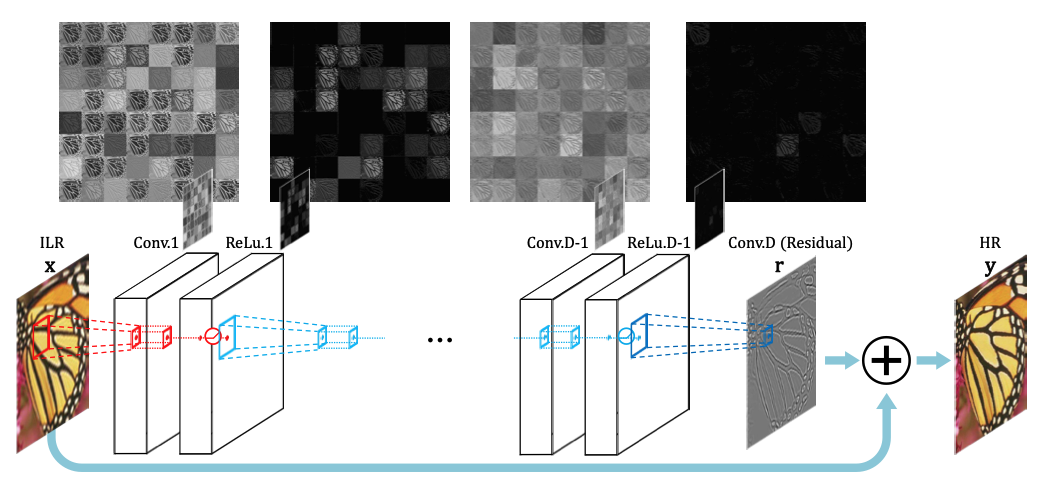
\includegraphics[width=\textwidth]{img/vdsr.png}
	\caption{VDSR architecture\cite{kim2015accurate}}
	\label{vdsr}
\end{figure*}
Very Deep CNN exploits a large number of layers to restore image and improve quality.
Its architecture includes a cascade of hidden layers which include small filters in equal number.\\
Each hidden layer has 64 filters and each of them as a dimension of 3x3.
The number of hidden layers is an hyperparameter.
The main idea behind this network is the implementation of residual learning. In the previous models, the exact copy of the input has to go through all layers until it reaches the output layer. This becomes an end-to-end relation between input  and output but this relationship, in a deep model, can create serious problems such as difficulty to train the network and vanishing/exploding gradients.
The input of VDSR mis the interpolated image \textit{\textbf{x}} and the target is the high resolution image \textit{\textbf{y}}.
Since \textit{\textbf{x}} and \textit{\textbf{y}} are pretty similar we can learn only the residual image $\textbf{r} = \textbf{y} - \textbf{x}$ .\\
After the generation of the output is possible to reconstruct the HR image summing the interpolated image with the residual.\\
The authors of the original paper have demonstrated that is possible to train this network, to learn Super Resolution, in  different scale factors using a dataset that contains images down-sampled in multiple scale factors.




\section{Experiments}
We have implemented these three networks using Python language and tools described above:
\begin{itemize}
	\item OpenCV: Images processing;
	\item Tensorflow: CNN building and training;
	\item Scikit-image : Metrics computation;
	\item Google Colab: Cloud computing service, although the free version is limited, the computing power is superior to our laptops due to the GPU computing
\end{itemize}
Our aim is to verify if the increase of complexity, in the architectures used, also brings a considerable increase on the performance in the SISR task.\\
We have measured performance using classical image compression metrics:
\begin{itemize}
	\item Mean Squared Error (MSE) : The mean of squared  difference between ground truth image pixels and restored image pixels. The lower the MSE, the better the quality of the reconstructed image.
	\item Peak Signal to Noise Ratio (PSNR) : Ratio between the maximum possible value and the value of distorsion in the image. Resolve the MSE problem, that is the dependence with the pixel scale. The higher the PSNR, the better the quality of the reconstructed image.
	\item Structural similarity (SSIM) : method that measures the perceptual difference between two similar images. Unlike PSNR, SSIM is based on visible structures in the image. The higher the SSIM, the better the quality of the reconstructed image.
\end{itemize}

In order to realize a fair comparison between the three models we trained all of them with T91 dataset but different data augmentation such as different number of patches extracted.\\
For SRCNN we extracted about 20000 patches, for FSRCNN the number increased to 30000 and for VDSR, the deeper network, we used 40000 patches.\\
All CNNs are trained with  Adam algorithm \cite{kingma2014adam} and we have done different trials with different learning rates, batch sizes and number of epochs.\\
In table \ref{param} we report final configurations.
\begin{table}[h!]
\begin{center}
	\begin{tabular}{|c| c| c| c| c|} 
		
		\hline
		& Layers & Learning rate & batch size & epochs \\ 
		\hline
		SRCNN & 3 & 0.001 & 256 & 400 \\
		\hline
		FSRCNN & 6 & 0.001 & 64 & 100\\
		\hline
		VDSR & 10 & 0.0001 & 64 & 50\\
		\hline
	\end{tabular}
\label{param}
\end{center}
\caption{Hyperparameters summary}
\end{table}

\begin{table*}
\begin{center}
	\begin{tabular}{|c| c| c| c| c| c| c| c| c| c|} 
		
		\hline
		Dataset & Scale & Bicubic  & SRCNN & FSRCNN & VDSR\\ 
		 &  & PSNR/SSIM/MSE &PSNR/SSIM/MSE & PSNR/SSIM/MSE & PSNR/SSIM/MSE \\ 
		\hline
		\multirow{3}{*}{Set5} & $\times2$ & 33.075/0.909/46.008 & 34.033/0.920/32.594 & \textcolor{red}{34.463}/\textcolor{red}{0.948}/\textcolor{red}{28.766} & 33.807/0.945/36.023 \\
		 									& $\times3$ & 28.286/0.824/142.542 & \textcolor{red}{29.027}/0.841/\textcolor{red}{110.992} & 28.941/\textcolor{red}{0.872}/114.039 & 28.766/0.870/ 122.674\\
		 									& $\times4$ & 26.332/0.771/ 227.509 & \textcolor{red}{26.933}/0.790/\textcolor{red}{186.851} & 26.479/0.808/213.039 & 26.736/\textcolor{red}{0.818}/201.497 \\
		\hline
		\multirow{3}{*}{Set14} & $\times2$ & 29.243/0.852/100.793 & \textcolor{red}{30.028}/0.854/91.442 & 29.991/\textcolor{red}{0.895}/\textcolor{red}{89.389} & 29.661/0.860/94.007 \\
											& $\times3$ & 24.896/0.728/267.894 & \textcolor{red}{25.678}/0.732/\textcolor{red}{240.882} & 25.333/\textcolor{red}{0.768}/246.676 &25.199/0.738/252.547 \\
											& $\times4$ &23.388/0.667/369.691 & \textcolor{red}{24.172}/0.672/\textcolor{red}{330.994} & 23.654/\textcolor{red}{0.697}/352.55 & 23.682/0.678/348.158 \\
		\hline
	\end{tabular}
\label{results}
\end{center}
\caption{Results. \textcolor{red}{Red color: Best performance}}
\end{table*}
IMMAGINI RISULTATI
\begin{figure*}[]
	\centering
	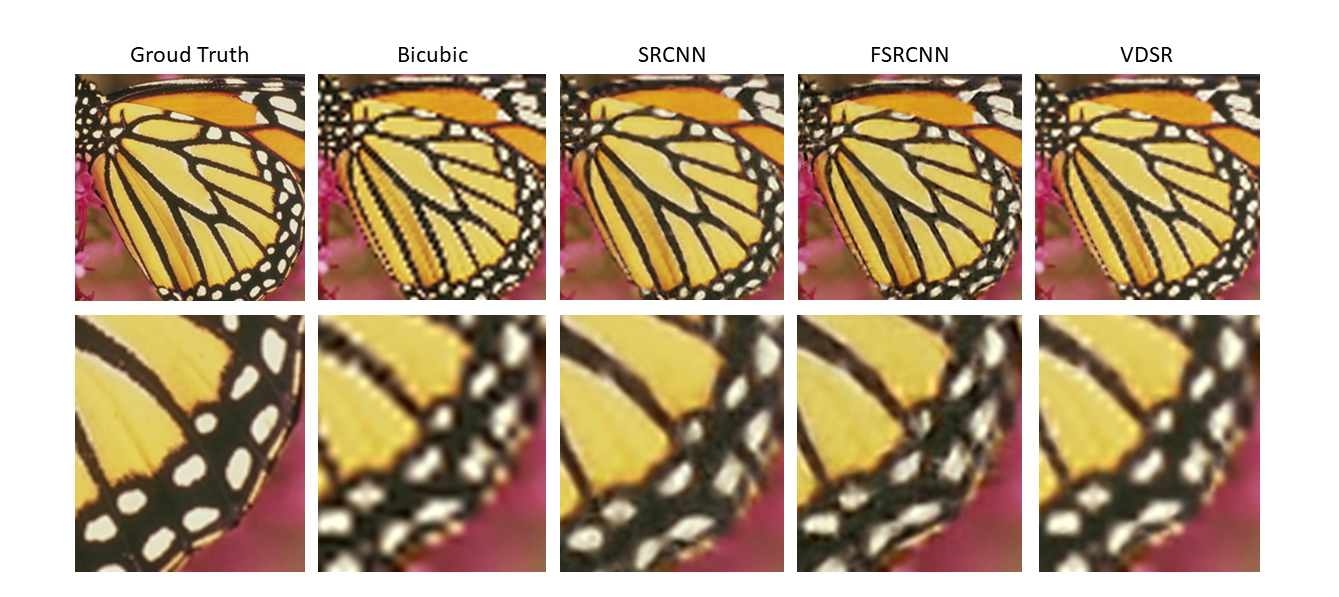
\includegraphics[width=\textwidth]{img/RESULTS.png}
	\caption{A graphical comparison of the restored images}
	\label{imgres}
\end{figure*}


\section{Conclusion}
We can say that we have achieved our goal, which is to demonstrate that more complex networks achieve better results.
Comparing our results with the various papers that we studied, we obtained lower PSNR and SSIM results for both the network output and the LR respect the original image, especially for factor scales other 2. We think it is due for use of anti aliasing in the preprocessing of the images used by the various papers.
Furthermore, the reconstructed images of the various networks, especially for factor scales equal to 4, are not very good, so the network was unable to reconstruct the high resolution image.
For SRCNN and FSRCNN we think it is due to an architecture
too easy. Also to compare the results the networks were trained with T91, which is a rather small dataset, so better performance could be obtained with larger datasets,however we were limited by Colab's ability.
The lack of data was felt more for VDSR which is a deeper network, however we were able to alleviate the effects by applying data argumentation.
In conclusion we liked working on this type of task, because it has never been seen before, even if it was difficult to understand the functioning of the various networks based on the papers of the creators. There are deeper convolutional networks and other more effective methods to have better performance in the Super Resolution task that we have not been able to implement due to computational limitations.

{\small
\bibliographystyle{ieee_fullname}
\bibliography{project_report_bib}
}

\end{document}
